\PassOptionsToPackage{unicode,pdfusetitle}{hyperref}
\PassOptionsToPackage{hyphens}{url}
\PassOptionsToPackage{dvipsnames,svgnames,x11names}{xcolor}

\documentclass[10pt,aspectratio=169]{beamer}

\usetheme{moloch}

\molochset{numbering=fraction}

% \setbeamertemplate{footline}[frame number]
% \setbeamertemplate{page number in head/foot}[appendixframenumber]

\usefonttheme{professionalfonts}

\usepackage{lmodern}
\usepackage{amssymb,amsmath,mathtools,amsthm}
\usepackage[T1]{fontenc}
\usepackage{textcomp} % provide euro and other symbols

\usepackage{pgfpages}

\usepackage{multirow}
\usepackage{csvsimple}
\usepackage{siunitx}

\usepackage{pifont}

% Use upquote if available, for straight quotes in verbatim environments
\usepackage{upquote}
\usepackage[]{microtype}
\UseMicrotypeSet[protrusion]{basicmath} % disable protrusion for tt fonts

\usepackage{xcolor}
\usepackage{xurl} % add URL line breaks if available
\usepackage{bookmark}
\usepackage{hyperref}
\hypersetup{%
  colorlinks = true,
  linkcolor  = Cyan4,
  filecolor  = Cyan4,
  citecolor  = SlateBlue4,
  urlcolor   = SlateBlue4
}

% tikz and pgfplots stuff
\usepackage{tikz}
\usetikzlibrary{arrows,shapes,positioning,intersections}
\usepackage{pgfplots}
\usepgfplotslibrary{external,colormaps}
\pgfplotsset{width=7cm,compat=1.18}
%\tikzexternalize

%\usepackage{subfig}
\usepackage{subcaption}
\usepackage{algorithm,algpseudocode}
\usepackage{booktabs}

% bibliography
\usepackage[citestyle=authoryear]{biblatex}
\addbibresource{references.bib}


% operators
\DeclareMathOperator*{\argmax}{arg\,max}
\DeclareMathOperator*{\argmin}{arg\,min}
\DeclareMathOperator{\E}{\text{E}}
\DeclareMathOperator{\var}{var}
\DeclareMathOperator{\cov}{cov}
\DeclareMathOperator{\sign}{sign}
\DeclareMathOperator{\card}{card}
\DeclareMathOperator{\cumsum}{cumsum}
\DeclareMathOperator*{\prox}{prox}

% macros
\newcommand{\pkg}[1]{\textsf{#1}}
\renewcommand{\vec}{\vectorsym}
\newcommand{\mat}{\matrixsym}
\newcommand{\du}{\mathrm{d}}

\makeatletter
\newcommand\notsotiny{\@setfontsize\notsotiny\@vipt\@viipt}
\makeatother



% title block
\title{Post-Doc Interview Presentation}
\author{Johan Larsson}
\institute{Department of Statistics, Lund University}
\date{\today}
\begin{document}

\maketitle

\begin{frame}[c]
  \frametitle{Outline}
  \tableofcontents
\end{frame}

\section{Coordinate Descent for SLOPE (Latest Work)}

\begin{frame}[c]
  \frametitle{Coordinate Descent for SLOPE}

  \begin{alertblock}{The Problem}
    SLOPE is a sparsity-inducing model with appealing properties, but the
    best algorithms (up til now) for solving SLOPE are slow.
  \end{alertblock}

  \begin{exampleblock}{Our Contribution}
    A hybrid algorithm based on coordinate descent (CD) and
    proximal gradient descent.
  \end{exampleblock}

  \pause

  A collaboration with Quentin Klopfenstein, Mathurin Massias, and Jonas Wallin.

  \begin{center}
    \hfill
    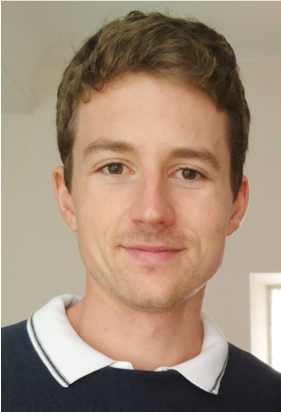
\includegraphics[height=2cm]{figures/quentin.png}
    \hfill
    
\includegraphics[height=2cm]{figures/mathurin.jpg}
    \hfill
    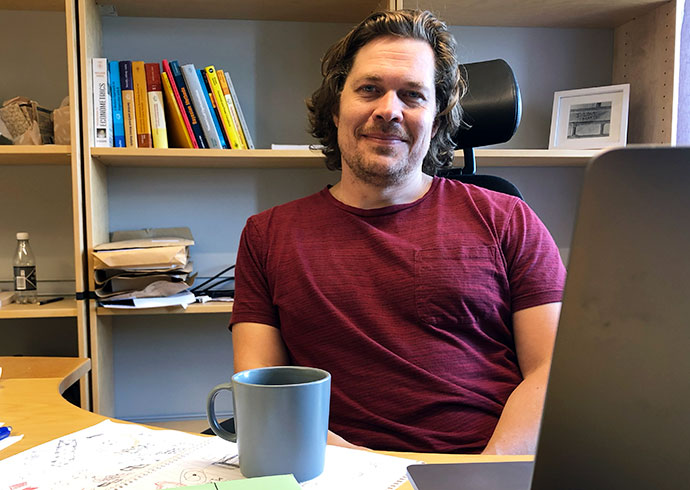
\includegraphics[height=2cm]{figures/jonas.jpg}
    \hfill
    \null
  \end{center}
\end{frame}

\begin{frame}[c]
  \frametitle{Sorted L-One Penalized Estimation (SLOPE)}

  For a design matrix \(X \in \mathbb{R}^{n \times p}\) and response vector \(y \in \mathbb{R}^n\), the solution to SLOPE is
  \[
    \beta^* \in \argmin_{\beta \in \mathbb{R}^p}
    \left\{P(\beta) =  \frac{1}{2} \norm{y - X \beta}^2 + J(\beta)\right\}
  \]
  where
  \begin{equation*}
    J(\beta) = \sum_{j=1}^p \lambda_j|\beta_{(j)}|
  \end{equation*}
  is the \alert{sorted \(\ell_1\) norm}, defined through
  \begin{equation}
    |\beta_{(1)}| \geq |\beta_{(2)}| \geq \cdots \geq |\beta_{(p)}|,
  \end{equation}
  with \(\lambda\) being a fixed non-increasing and non-negative sequence.

  \pause

  \begin{block}{Special Cases}
    \begin{itemize}
      \item \(\lambda_1 = \cdots = \lambda_p \rightarrow \ell_1\) (the lasso penalty)
      \item \(\lambda_1 > \lambda_2 = \cdots = \lambda_p = 0 \rightarrow \ell_\infty\)
    \end{itemize}
  \end{block}

\end{frame}

\begin{frame}[c]
  \frametitle{Properties}

  \begin{columns}
    \begin{column}{0.45\textwidth}
      SLOPE has many appealing properties:
      \begin{itemize}
        \item \alert{Clustering}~\parencite{bogdan2022,schneider2020a,figueiredo2016}
        \item \alert{Control of false discovery rate}~\parencite{bogdan2013,bogdan2015}
        \item \alert{Recovery of sparsity and ordering patterns}~\parencite{bogdan2022}
        \item \alert{Convexity}
      \end{itemize}

      \onslide<2->{\bfseries{So why isn't SLOPE more popular?}}

    \end{column}
    \begin{column}{0.45\textwidth}
      \begin{figure}
        \centering
        \pgfplotsset{width=7cm,height=7cm}
        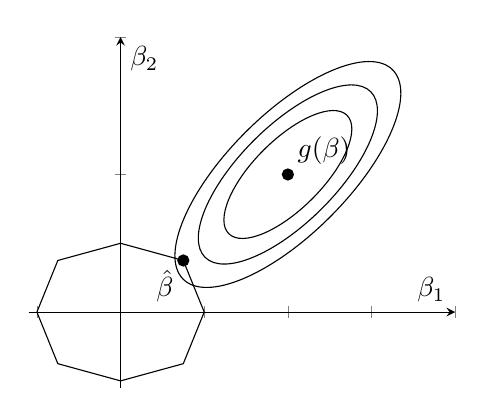
\begin{tikzpicture}
\begin{axis}[
    xlabel = \(\beta_1\),
    ylabel = \(\beta_2\),
    ymin = -1.1,
    ymax = 4,
    xmin = -1.1,
    xmax = 4,
    axis lines = center,
    yticklabels={,,},
    xticklabels={,,}
]
\draw[rotate around={45:(2,2)}] (2,2) ellipse (1 and 0.5);
\draw[rotate around={45:(2,2)}] (2,2) ellipse (1.4 and 0.7);
\draw[rotate around={45:(2,2)}] (2,2) ellipse (1.77 and 0.87);

\addplot[]
    coordinates {
    	(-1,0)
    	(-0.75, 0.75)
    	(0,1)
    	(0.75,0.75)
    	(1,0)
    	(0.75,-0.75)
    	(0,-1)
    	(-0.75,-0.75)
    	(-1,0)
    };
\addplot [only marks, mark=*] coordinates {(2,2)};
\node [above right,black] at (2,2) {$g(\beta)$};

\addplot [only marks, mark=*] coordinates { (0.75,0.75) };
\node [below left] at (0.75,0.75) {$\hat\beta$};
\end{axis}
\end{tikzpicture}
        \caption{%
          The SLOPE solution seen as a constrained problem.
        }
      \end{figure}

    \end{column}
  \end{columns}

\end{frame}

% \begin{frame}[c]
%   \frametitle{Why Is SLOPE Not More Popular?}
%   % \framesubtitle{Why doesn't everyone already use SLOPE?}
%
%   \begin{columns}
%     \begin{column}{0.45\textwidth}
%       \begin{itemize}
%         \item<1-> The lasso is much more popular than SLOPE.
%         \item<2-> One reason is that current state-of-the-art algorithms for fitting the lasso are much faster.
%               \medskip
%
%               \textbf{Example}: Fitting the \texttt{bcTCGA} data set with the R-package SLOPE takes
%               43 seconds versus 0.14 seconds for glmnet (lasso).
%       \end{itemize}
%
%     \end{column}
%     \begin{column}{0.45\textwidth}
%       \begin{figure}
%         \centering
%         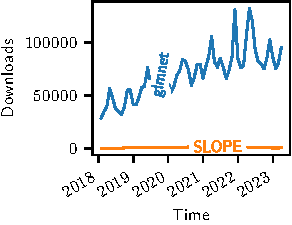
\includegraphics[]{figures/cran-stats.pdf}
%         \caption{%
%           CRAN download statistics for the SLOPE and glmnet (lasso) packages.
%         }
%       \end{figure}
%     \end{column}
%   \end{columns}
% \end{frame}

\begin{frame}
  \frametitle{Coordinate Descent}

  \begin{columns}[c]
    \begin{column}{0.45\textwidth}
      \begin{itemize}
        \item<1-> Partly because the best solvers for the lasso use coordinate descent.
        \item<2-> Simple optimization method: at each iteration, update a single coordinate (coefficient).
      \end{itemize}
    \end{column}
    \begin{column}{0.45\textwidth}
      \begin{figure}[htpb]
        \centering
        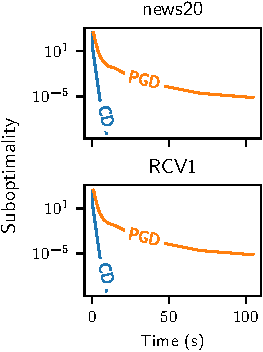
\includegraphics[]{figures/cd-vs-pgd.pdf}
        \caption{%
          Coordinate descent versus proximal gradient descent for the lasso.
        }
      \end{figure}
    \end{column}
  \end{columns}
\end{frame}

\begin{frame}
  \frametitle{Coordinate Descent and Inseparability}
  \begin{columns}
    \begin{column}{0.45\textwidth}
      \begin{itemize}
        \item<1-> Unfortunately, we cannot use basic coordinate descent for SLOPE since the
              sorted \(\ell_1\) norm is \alert{inseparable}:
              \[
                J(\beta) = \sum_{j=1}^p \lambda_j |\beta_{(j)}|.
              \]
        \item<2-> But if we fix the clusters, we have separability and can solve SLOPE using coordinate descent.
        \item<3-> \bfseries{Idea:} Alternate between gradient descent steps (identify the clusters) and
              coordinate descent steps \alert{on the clusters} (converge quickly).
      \end{itemize}
    \end{column}
    \begin{column}{0.45\textwidth}
      \begin{figure}[htpb]
        \centering
        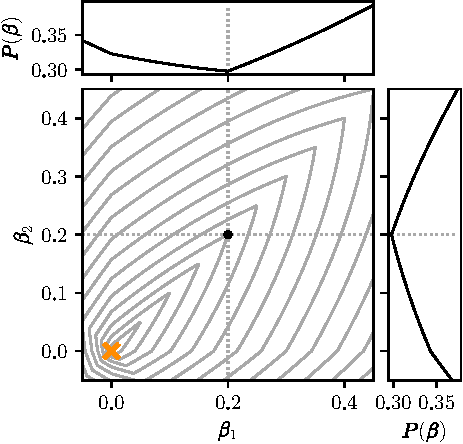
\includegraphics[height=5.5cm]{figures/naive-cd-stuck.pdf}
        \caption{A \emph{naive} coordinate descent algorithm cannot advance from the
          current iterate (\ding{108}) to reach the optimum ({\color{orange}\ding{54}}).}
      \end{figure}
    \end{column}
  \end{columns}

\end{frame}

% \begin{frame}[c]
%   \frametitle{Clusters Are Not Known In Advance}
%
%   If we fix the clusters, the problem becomes separable and we could solve it using coordinate descent. And if we knew what the optimal clusters were, this would be a solution to the problem.
%   % \[
%   %   \min_{z \in \mathbb{R}^{m^*}}\bigg(
%   %   \frac{1}{2} \Big\lVert y - X \sum_{i=1}^{m^*} \sum_{j \in \mathcal{C}_i^*} z_i \sign(\beta_j^*) e_j \Big\rVert^2 + \sum_{i=1}^{m^*} | z_i | \sum_{j \in \mathcal{C}_i^*} \lambda_j
%   %   \bigg),
%   % \]
%
%   \pause
%
%
% \end{frame}

\begin{frame}[c]
  \frametitle{Hybrid Algorithm}

  \begin{itemize}
    \item Every \(v\)th iteration, take a full proximal gradient step.
          This allows clusters to split (or merge).
    \item At all other iterations, take coordinate descent steps on the clusters.
  \end{itemize}

  \pause

  \begin{figure}[htpb]
    \centering
    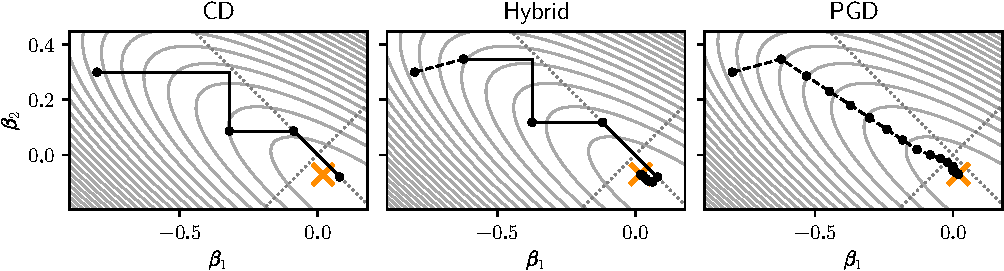
\includegraphics[width=\textwidth]{figures/illustration_solvers.pdf}
    \caption{%
      Our algorithm (hybrid) is a combination of CD and PGD.
    }
  \end{figure}

\end{frame}

\begin{frame}
  % \frametitle{Experiments: Real Data}

  \begin{figure}[htpb]
    \centering
    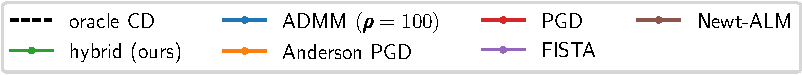
\includegraphics[scale=0.6]{figures/real_legend.pdf}
    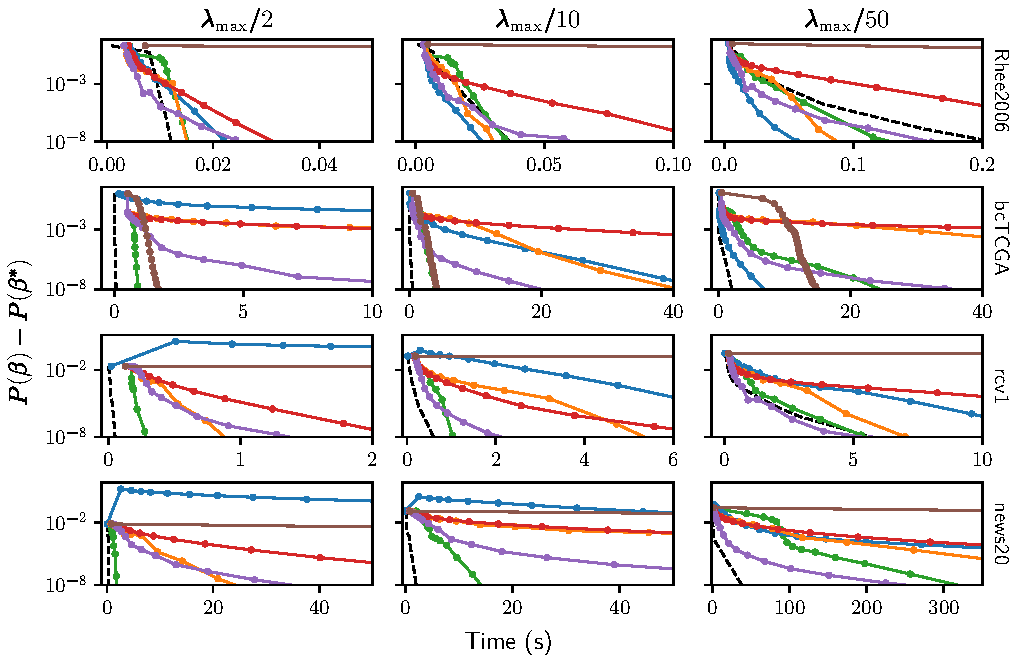
\includegraphics[scale=0.6]{figures/real.pdf}
    \caption{%
      Benchmarks on real data
    }
  \end{figure}
\end{frame}

% \begin{frame}
%   \frametitle{Experiments: Simulated Data}
%
%   \begin{figure}[htpb]
%     \centering
%     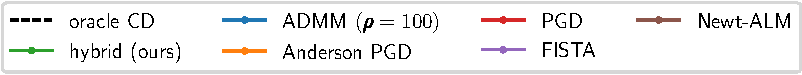
\includegraphics[scale=0.55]{figures/simulated_legend.pdf}
%     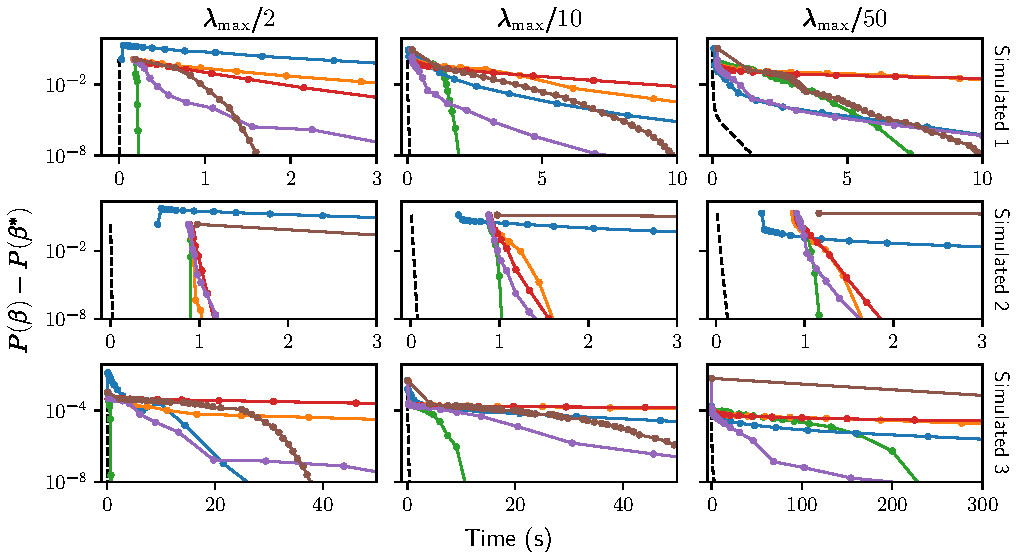
\includegraphics[scale=0.6]{figures/simulated.pdf}
%     \caption{%
%       Benchmarks on simulated data. Scenario 1: \(n = 200\) and \(p = 20\,000\),
%       \(X\). Scenario 2: \(n = 20\,000\) and \(p = 200\). Scenario 3: \(n = 200\),
%       \(p = 200\,000\), and sparse \(X\).
%     }
%   \end{figure}
% \end{frame}

\section{Previous Work}

\begin{frame}[c]
  \frametitle{The Strong Screening Rule for SLOPE}

  \begin{columns}
    \begin{column}{0.45\textwidth}
      Basic idea:
      \begin{itemize}
        \item When \(p \gg n\), SLOPE and lasso solutions have small support.
        \item If we can estimate the support (before fitting the model), we save a lot of time.
        \item If the screening method is cheap, we have a net gain.
      \end{itemize}
      \pause
      A game-changer for the lasso. But for SLOPE, there were no screening rules before our work~\parencite{larsson2020b}.
    \end{column}
    \pause
    \begin{column}{0.45\textwidth}
      \begin{figure}
        \centering
        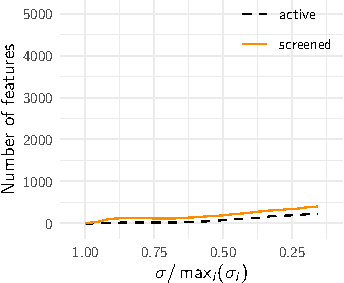
\includegraphics{figures/strong-efficiency-gaussian.pdf}
        \caption{%
          Number of features screened along the SLOPE path for for a data set with 200 observations and 5000 features.
        }
      \end{figure}
    \end{column}
  \end{columns}
\end{frame}

% \begin{frame}[c]
%   \begin{figure}[htpb]
%     \centering
%     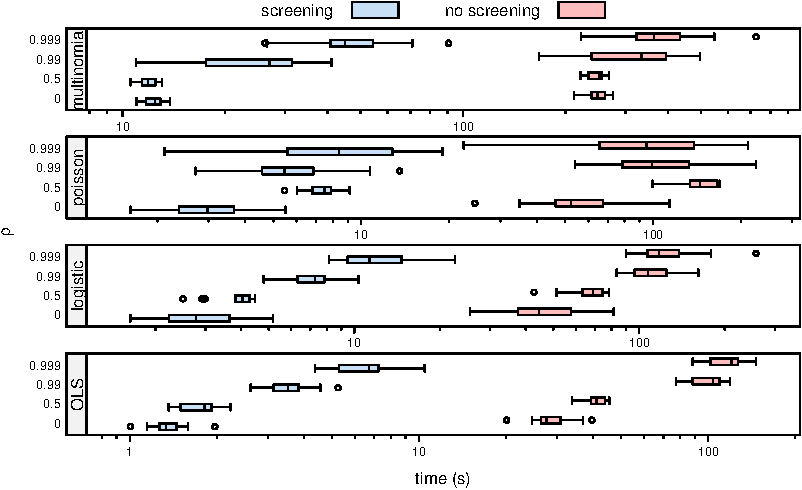
\includegraphics[width=0.8\textwidth]{figures/strong-rule-performance.pdf}
%     \caption{%
%       Performance for the strong screening rule for solving sorted \(\ell_1\)-penalized least squares and logistic regression problems.
%     }
%   \end{figure}
% \end{frame}

\begin{frame}[c]
  \frametitle{The Hessian Screening Rule}
  \begin{columns}
    \begin{column}{0.4\textwidth}
      In this paper~\parencite{larsson2022b} we continued our work on screening rules, but for the lasso instead.\medskip

      \textbf{Our contribution:} a new rule that uses second-order information to better predict the support along the regularization path.
    \end{column}
    \begin{column}{0.5\textwidth}
      \begin{figure}
        \centering
        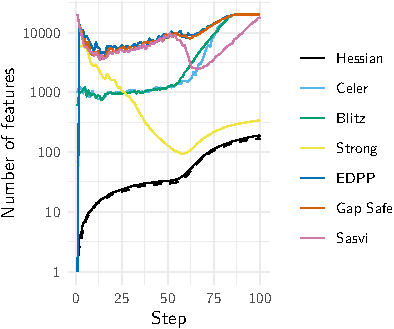
\includegraphics{figures/hessian-simulateddata-efficiency.pdf}
        \caption{%
          Number of features (predictors) screened along the SLOPE path for designs with varying correlation \((\rho)\).
        }
      \end{figure}
    \end{column}
  \end{columns}

\end{frame}


\begin{frame}[c]
  \frametitle{Benchopt}

  Benchopt~\parencite{moreau2022a} strives to make benchmarking easy, transparent, and reproducible.

  \begin{figure}[htpb]
    \centering
    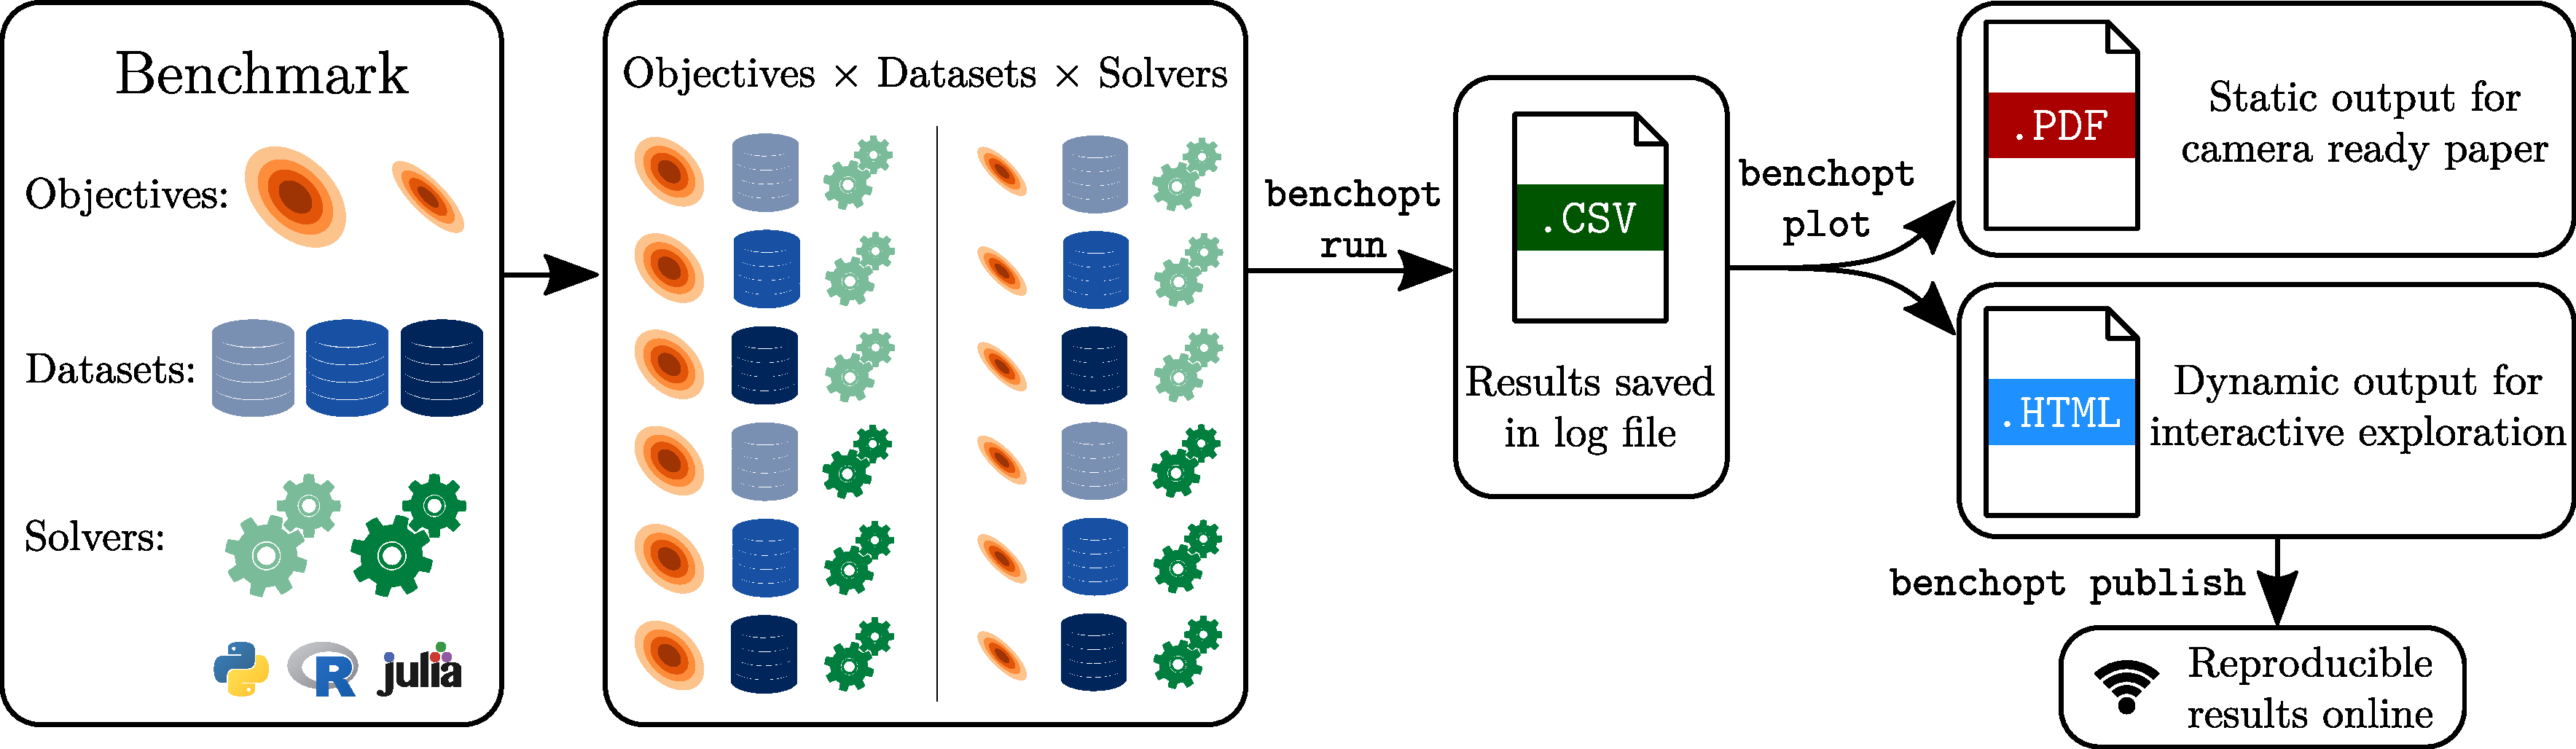
\includegraphics[width=\textwidth]{figures/benchopt_schema.pdf}
    \caption{%
      How Benchopt works.
    }
  \end{figure}
\end{frame}

\section{Ongoing Work}

\begin{frame}[c]
  \frametitle{Regularization And Normalization}
  \begin{columns}
    \begin{column}{0.45\textwidth}
      \begin{itemize}
        \item Normalization is essential for regularized methods, but there is almost no work on the topic.
        \item What effects do different types of normalization have on the solutions of regularized methods?
      \end{itemize}
    \end{column}
    \begin{column}{0.45\textwidth}
      \begin{figure}[htpb]
        \centering
        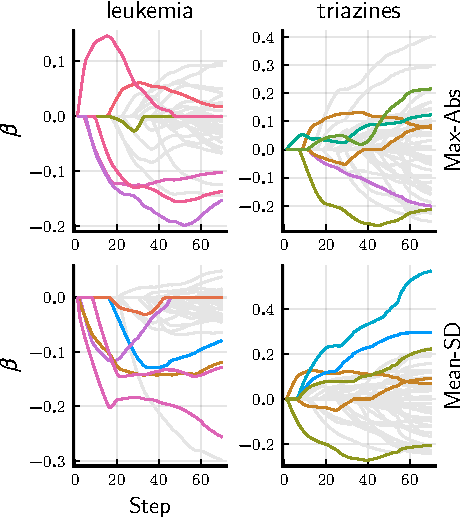
\includegraphics[width=5.5cm]{figures/realdata_paths.pdf}
        \caption{%
          Lasso paths for two types of normalization.
        }
      \end{figure}
    \end{column}
  \end{columns}
\end{frame}

\begin{frame}[standout]
  Thank you!
\end{frame}

% \setbeamertemplate{frame numbering}[none]

\appendix

\begin{frame}[allowframebreaks]{References}
  % \bibliographytrue
  \printbibliography[heading=none]
\end{frame}

\begin{frame}
  \frametitle{Coordinate Descent Steps}

  When updating the \(k\)th cluster, we let
  \begin{equation*}
    \beta_i(z) =
    \begin{cases}
      \mathrm{sign}(\beta_i) z   , & \text{if } i \in \mathcal{C}_k, \\
      \beta_i,                     & \text{otherwise}.
    \end{cases}
  \end{equation*}

  \pause

  Minimizing the objective in this direction amounts to solving the following
  one-dimensional problem:
  \[
    \min_{z \in \mathbb{R}} \Big(
    G(z) = P(\beta(z))  = \frac{1}{2} \lVert y - X \beta(z)\rVert^2 + H(z)
    \Big),
  \]
  where
  \begin{equation*}
    H(z) = |z| \sum_{j \in \mathcal{C}_k} \lambda_{(j)^-_z}
    + \sum_{j \notin \mathcal{C}_k} |\beta_j| \lambda_{(j)^-_z}
  \end{equation*}
  is the \emph{partial sorted \(\ell_1\) norm} with respect to the \(k\)-th cluster and where we write \(\lambda_{(j)^-_z}\) to indicate that the inverse sorting permutation \((j)^-_z\)
  is defined with respect to \(\beta(z)\).
\end{frame}


\begin{frame}
  \frametitle{The Partial Sorted \(\ell_1\) Norm}

  \begin{figure}[htpb]
    \centering
    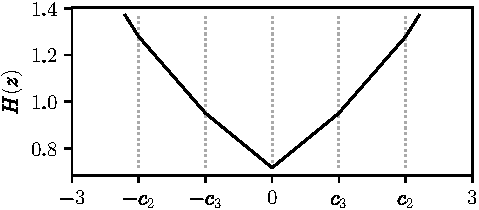
\includegraphics[scale=0.8]{figures/partial_slope.pdf}
    \caption{%
    The partial sorted \(\ell_1\) norm with \(\beta = [-3,1,3,2]^T\), \(k = 1\), and so
    \(c_1, c_2, c_3 = (3,2,1)\).
    }
  \end{figure}
\end{frame}

\begin{frame}
  \frametitle{How Do We Minimize Over One Cluster?}

  \begin{columns}
    \begin{column}{0.35\textwidth}
      The optimality condition, using the directional derivative, is
      \[
        \forall \delta \in \{-1, 1\}, \quad G'(z; \delta) \geq 0,
      \]
      with
      \[
        \begin{multlined}
          G'(z; \delta)  \\= \delta \sum_{j \in \mathcal{C}_k} X_{:j}^\top(X\beta(z) - y) \\
          + H'(z; \delta).
        \end{multlined}
      \]
    \end{column}
    \begin{column}{0.55\textwidth}
      \begin{figure}
        \centering
        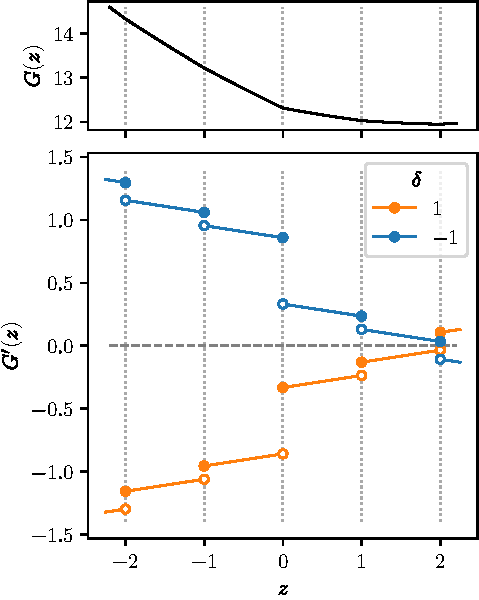
\includegraphics[width=5.3cm]{figures/directional-derivative.pdf}
        \caption{%
          \(G\) and its directional derivative \(G'( \cdot ; \delta)\).
        }
      \end{figure}
    \end{column}
  \end{columns}
\end{frame}

\begin{frame}
  \frametitle{The SLOPE Thresholding Operator}

  \begin{figure}[htpb]
    \centering
    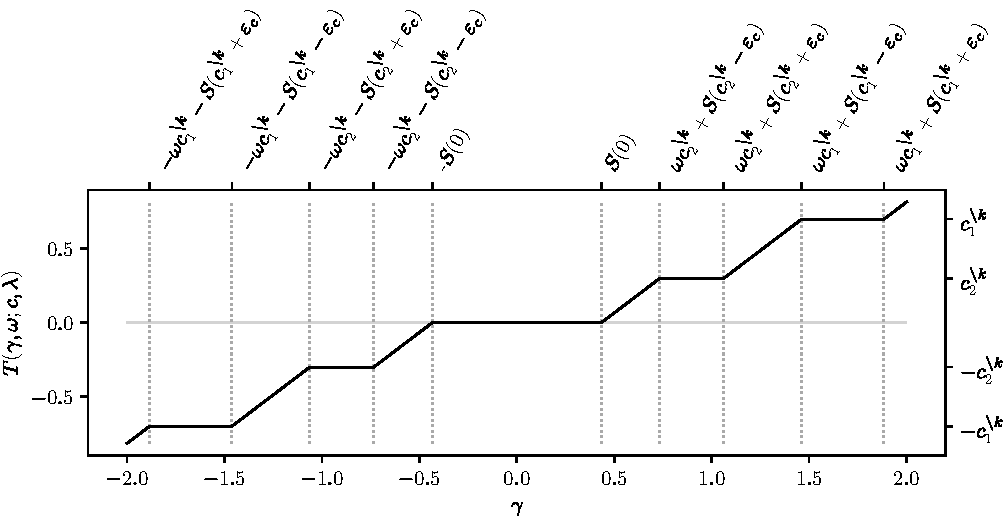
\includegraphics[width=0.9\textwidth]{figures/slope-thresholding.pdf}
    \caption{%
      The SLOPE Thresholding Operator
    }
  \end{figure}
\end{frame}

\end{document}
